\chapter{Computer Architecture}
\label{ch:arch}

Computer architecture is the level above circuits: how a processor is organized to run programs quickly. Interviewers for hardware internships often ask about it (``what are the stages of a five-stage pipeline?''), and NVIDIA hardware tests have included cache and memory-timing calculations. This chapter gives the essentials.

\section{What a processor does}

A processor runs a program stored in memory as a list of \term{instructions}. The set of instructions a processor understands, and how they are encoded, is its \term{instruction set architecture} (ISA): x86 in most PCs, ARM in phones, RISC-V in many new designs. A processor holds a small number of fast \term{registers}, and a \term{program counter} (PC) that points at the next instruction. Each instruction goes through the same cycle:
\begin{enumerate}
  \item \textbf{Fetch} the instruction at the PC from memory.
  \item \textbf{Decode} it: what operation, which registers.
  \item \textbf{Execute}: do the arithmetic, compare, or compute an address.
  \item Access \textbf{memory} if it is a load or store.
  \item \textbf{Write back} the result to a register, and move the PC to the next instruction (or the branch target).
\end{enumerate}

Instructions come in a few families: arithmetic and logic (\code{add r1, r2, r3}), memory (\code{load r1, 8(r2)} and \code{store}), and control flow (\code{branch if equal}, \code{jump}).

\section{Measuring performance}

\begin{bigidea}
The \textbf{processor performance equation}:
\[
  \text{execution time} = \text{instruction count} \times \text{CPI} \times \text{clock period},
\]
where CPI is the average number of clock cycles per instruction. Every architecture idea attacks one of these three factors.
\end{bigidea}

\begin{worked}{run time}
A program executes $10^9$ instructions with an average CPI of 1.5 on a 2\,GHz processor (0.5\,ns period). Time $= 10^9 \times 1.5 \times 0.5\times10^{-9} = 0.75$\,s.
\end{worked}

\section{The five-stage pipeline}

A simple processor could do all five steps of one instruction in one long clock cycle. A \term{pipelined} processor instead splits the steps into stages separated by registers (Section~\ref{sec:pipelining}), and works on five different instructions at once, one in each stage, like an assembly line.

\begin{onoa}
``What are the stages in a five-stage pipelined processor?'' is a reported NVIDIA hardware intern interview question. The classic answer: \textbf{IF} (instruction fetch), \textbf{ID} (instruction decode and register read), \textbf{EX} (execute, using the ALU), \textbf{MEM} (memory access for loads and stores), \textbf{WB} (write back to the register file).
\end{onoa}

\begin{figure}[h]
\centering
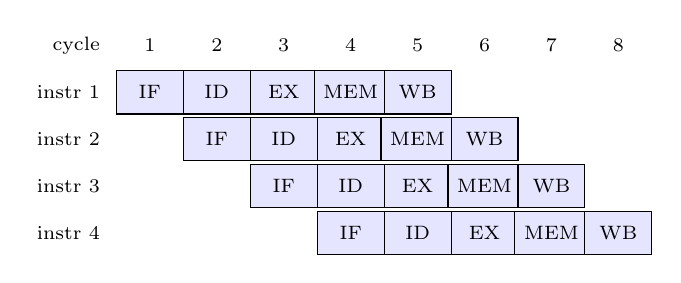
\begin{tikzpicture}[scale=0.85, st/.style={draw,minimum width=0.85cm,minimum height=0.55cm,font=\scriptsize}]
  \foreach \c in {1,...,8} \node[font=\scriptsize] at (\c,0.7) {\c};
  \node[font=\scriptsize,anchor=east] at (0.4,0.7) {cycle};
  \foreach \i/\name in {0/{instr 1},1/{instr 2},2/{instr 3},3/{instr 4}} {
    \node[font=\scriptsize,anchor=east] at (0.4,-\i*0.7) {\name};
    \foreach \s [count=\k from 0] in {IF,ID,EX,MEM,WB}
      \node[st,fill=blue!10] at (\i+\k+1,-\i*0.7) {\s};
  }
\end{tikzpicture}
\caption{A five-stage pipeline. Once full, one instruction finishes every cycle, even though each takes five cycles.}
\label{fig:pipeline}
\end{figure}

Each instruction still takes five cycles (its latency), but a new one finishes every cycle (the throughput), so the ideal CPI is 1 and the clock can be about five times faster than a single-cycle design.

\begin{worked}{pipeline speedup}
A non-pipelined processor runs at 2.5\,GHz but needs 5 cycles per instruction (CPI = 5). A pipelined version runs at 2\,GHz (pipeline registers add overhead) with CPI = 1.

Non-pipelined: $2.5\times10^9/5 = 0.5$ billion instructions per second. Pipelined: $2\times10^9/1 = 2$ billion. Throughput speedup: $2/0.5 = 4\times$.
\end{worked}

\section{Hazards}

Overlapping instructions causes three kinds of trouble, called \term{hazards}.

\paragraph{Structural hazards.} Two instructions need the same hardware in the same cycle (for example, one memory port for both fetching and loading). Fixed by duplicating hardware, such as separate instruction and data caches.

\paragraph{Data hazards.} An instruction needs a result that an earlier instruction has not yet written back:
\begin{lstlisting}
add r1, r2, r3     # r1 is written in WB (cycle 5)
sub r4, r1, r5     # but sub reads r1 in ID (cycle 3)
\end{lstlisting}
The fix is \term{forwarding} (or bypassing): send the result straight from the end of the EX stage to the input of the next instruction's EX stage, without waiting for write-back. Forwarding fixes most data hazards with no delay.

One case it cannot fully fix is the \term{load-use hazard}: a load's data only arrives at the end of MEM, too late for an instruction right behind it that needs it in EX. The pipeline must \term{stall} (insert a bubble) for one cycle. Compilers reorder instructions to put something useful in that slot.

\paragraph{Control hazards.} After a branch, the processor does not know which instruction comes next until the branch is resolved, but the pipeline keeps fetching. If it guessed wrong, the wrongly fetched instructions must be \term{flushed}, wasting cycles (the \term{branch penalty}). \term{Branch prediction} guesses the outcome: simple predictors remember each branch's recent behavior (for example with 2-bit saturating counters), and a branch target buffer remembers where it jumps. Modern predictors are right well over 90\% of the time.

\section{Amdahl's law}

Speeding up one part of a task only helps as much as that part matters. If a fraction $p$ of the work is sped up by a factor $s$:
\[
  \boxed{\text{overall speedup} = \frac{1}{(1 - p) + p/s}}
\]

\begin{worked}{parallel speedup}
80\% of a program can run in parallel on 16 cores. Speedup $= 1/(0.2 + 0.8/16) = 1/0.25 = 4$. Even with infinitely many cores, the speedup can never exceed $1/0.2 = 5$: the serial 20\% sets the ceiling.
\end{worked}

\section{The memory hierarchy}

Processors are far faster than DRAM. Waiting about 100\,ns for every memory access would waste hundreds of clock cycles each time. The solution is a hierarchy of memories, small and fast near the processor, large and slow further away:

\begin{center}
\begin{tabular}{lll}
\toprule
Level & Typical size & Typical access time (approximate) \\
\midrule
Registers & hundreds of bytes to kilobytes & under 1\,ns \\
L1 cache (SRAM) & tens of KB & about 1\,ns \\
L2 cache & hundreds of KB to a few MB & a few ns \\
L3 / last-level cache & many MB & 10--40\,ns \\
DRAM & gigabytes & 50--100\,ns \\
SSD (flash) & terabytes & about 100\,$\mu$s \\
\bottomrule
\end{tabular}
\end{center}

This works because programs have \term{locality}:
\begin{itemize}
  \item \textbf{Temporal locality}: data used recently is likely to be used again soon (loop variables).
  \item \textbf{Spatial locality}: data near recently used data is likely to be used soon (array elements in order).
\end{itemize}

\section{How a cache works}

A cache stores copies of recently used memory in fixed-size blocks called \term{lines} (often 64 bytes; fetching a whole line exploits spatial locality). To find whether an address is in the cache, the address is split into three fields:
\[
  \underbrace{\text{tag}}_{\text{which line is this?}} \;\big|\; \underbrace{\text{index}}_{\text{which set to look in}} \;\big|\; \underbrace{\text{offset}}_{\text{which byte in the line}}
\]
\begin{itemize}
  \item \textbf{Offset} bits $= \log_2(\text{line size})$.
  \item \textbf{Index} bits $= \log_2(\text{number of sets})$.
  \item \textbf{Tag} bits $=$ address bits $-$ index bits $-$ offset bits. Each line stores its tag so the cache can check whether it holds the right address, plus a \term{valid} bit and usually a \term{dirty} bit.
\end{itemize}

\paragraph{Associativity.} In a \term{direct-mapped} cache, each address can go in exactly one line. In an \term{$N$-way set-associative} cache, each address maps to one \emph{set} of $N$ lines and can go in any of them. In a \term{fully associative} cache, it can go anywhere. More associativity means fewer conflicts but more tags to compare in parallel. When a set is full, a \term{replacement policy} (usually least recently used, LRU, or an approximation) picks a line to evict.

\paragraph{Writes.} A \term{write-through} cache sends every write on to the next level immediately. A \term{write-back} cache only updates its own copy and marks the line \emph{dirty}, writing it back when it is evicted, which saves bandwidth.

\paragraph{Why misses happen (the three Cs).} \textbf{Compulsory} misses: the first access to a line. \textbf{Capacity} misses: the working data does not fit. \textbf{Conflict} misses: too many addresses map to the same set, even though the cache has room elsewhere (eliminated by full associativity).

\begin{worked}{address fields and tag-array size}
A 1\,MB, 4-way set-associative cache has 64-byte lines and 32-bit addresses. Each line stores its tag plus a valid bit and a dirty bit. How big is the tag array?

Lines: $2^{20}/2^6 = 2^{14} = 16{,}384$. Sets: $16{,}384/4 = 4096 = 2^{12}$.
Offset: 6 bits. Index: 12 bits. Tag: $32 - 12 - 6 = 14$ bits.
Bits per line: $14 + 1 + 1 = 16$. Tag array: $16{,}384 \times 16 = 262{,}144$ bits $= 32$\,KB.
\end{worked}

\section{Average memory access time}

\begin{bigidea}
\[
  \text{AMAT} = \text{hit time} + \text{miss rate} \times \text{miss penalty}.
\]
With two levels, the L1 miss penalty is itself the AMAT of L2:
\[
  \text{AMAT} = t_{L1} + m_{L1}\,\big(t_{L2} + m_{L2}\,t_{mem}\big),
\]
where $m_{L2}$ is the \emph{local} miss rate of L2 (the fraction of L2 accesses that miss).
\end{bigidea}

\begin{worked}{a two-level AMAT}
L1 hits 80\% of the time and L2 hits 40\% of the accesses that reach it. Access times are 10\,ns for L1, 30\,ns for L2 and 100\,ns for memory.
\[
  \text{AMAT} = 10 + 0.2\,(30 + 0.6 \times 100) = 10 + 0.2 \times 90 = 28~\text{ns}.
\]
\end{worked}

\begin{trap}
Some questions state each level's time as the \emph{total} time for an access served at that level, not the extra time added on a miss. Then the answer is a weighted average of where accesses are served: $0.8 \times 10 + 0.2 \times 0.4 \times 30 + 0.2 \times 0.6 \times 100 = 8 + 2.4 + 12 = 22.4$\,ns. Read the wording to decide which model the question uses, and say which one you assumed.
\end{trap}

\begin{worked}{memory stalls and CPI}
A processor has a base CPI of 1.0. 30\% of instructions are loads or stores, their L1 miss rate is 2\%, and a miss costs 200 cycles. Memory stall cycles per instruction: $0.3 \times 0.02 \times 200 = 1.2$. Effective CPI: $1.0 + 1.2 = 2.2$. The memory system more than doubles the run time, which is why caches are worth so much silicon. To compare two memory systems (for example, L3 only versus L2 plus L3), compute the effective CPI for each and take the ratio.
\end{worked}

\section{Virtual memory}

Programs use \term{virtual addresses}; the hardware translates them to \term{physical addresses} in DRAM. Memory is divided into \term{pages}, typically 4\,KB. A per-process \term{page table} maps virtual page numbers to physical page numbers; the offset within the page (the low 12 bits for 4\,KB pages) is unchanged by translation. A \term{translation lookaside buffer} (TLB), a small cache of recent translations, makes this fast. Accessing a page that is not in memory causes a \term{page fault}, handled by the operating system.

This is why ``are two addresses on the same 4\,KB page?'' (Section~\ref{sec:bitops}) is a natural hardware question: same page means same translation.

\section{Endianness}

A 32-bit value occupies 4 bytes in memory. A \term{little-endian} machine (x86, most ARM and RISC-V systems) stores the least significant byte at the lowest address; a \term{big-endian} machine stores the most significant byte first. The value \code{0x12345678} stored at address \code{0x100}:
\begin{center}
\begin{tabular}{lcccc}
\toprule
Address & \code{0x100} & \code{0x101} & \code{0x102} & \code{0x103} \\
\midrule
Little-endian & \code{78} & \code{56} & \code{34} & \code{12} \\
Big-endian & \code{12} & \code{34} & \code{56} & \code{78} \\
\bottomrule
\end{tabular}
\end{center}

\section{Multiple cores}

A chip with several cores, each with its own cache, must keep the caches \term{coherent}: if one core writes a value, other cores must not keep reading a stale copy. Coherence protocols such as MESI track whether each cached line is Modified, Exclusive, Shared or Invalid, and invalidate other copies when one core writes.

\section{Summary}

\begin{itemize}
  \item Execution time $=$ instruction count $\times$ CPI $\times$ clock period.
  \item Five-stage pipeline: IF, ID, EX, MEM, WB. Ideal CPI of 1.
  \item Hazards: structural (duplicate hardware), data (forwarding; load-use needs a stall), control (branch prediction, flush).
  \item Amdahl: speedup $= 1/((1-p) + p/s)$; the serial part sets the limit.
  \item Caches exploit temporal and spatial locality. Address $=$ tag $|$ index $|$ offset.
  \item AMAT $=$ hit time $+$ miss rate $\times$ miss penalty, applied level by level.
  \item Virtual memory translates pages (4\,KB); the TLB caches translations.
  \item Little-endian stores the least significant byte first.
\end{itemize}

\section{Exercises}

\begin{enumerate}
  \item A program runs $2\times10^9$ instructions at CPI 1.2 on a 3\,GHz processor. How long does it take?
  \item Name the five stages of the classic pipeline and say what each does.
  \item Why does a load followed immediately by an instruction using its result need a stall, even with forwarding?
  \item 90\% of a task is parallel. What is the speedup on 10 cores? The maximum on unlimited cores?
  \item A 32\,KB direct-mapped cache has 64-byte lines and 32-bit addresses. Find the offset, index and tag widths.
  \item A cache has a 1\,ns hit time, 5\% miss rate and 100\,ns miss penalty. Find the AMAT.
  \item Which kind of miss does full associativity eliminate?
  \item Show how \code{0xA1B2C3D4} is stored at address 0 in a little-endian machine.
  \item Base CPI 1.0, 40\% loads/stores, 5\% miss rate, 100-cycle penalty. What is the effective CPI?
\end{enumerate}

\subsection*{Answers}
\begin{enumerate}
  \item $2\times10^9 \times 1.2 / (3\times10^9) = 0.8$\,s.
  \item IF fetches the instruction; ID decodes it and reads registers; EX computes in the ALU; MEM reads or writes data memory; WB writes the result to the register file.
  \item The loaded value is only available at the end of MEM, but the next instruction needs it at the start of its EX stage, which happens in the same cycle; it must wait one cycle.
  \item $1/(0.1 + 0.09) \approx 5.3$. Maximum $1/0.1 = 10$.
  \item Offset 6 bits; lines $= 2^{15}/2^6 = 512$, so index 9 bits; tag $32 - 9 - 6 = 17$ bits.
  \item $1 + 0.05 \times 100 = 6$\,ns.
  \item Conflict misses.
  \item Address 0: \code{D4}, 1: \code{C3}, 2: \code{B2}, 3: \code{A1}.
  \item $1.0 + 0.4 \times 0.05 \times 100 = 3.0$.
\end{enumerate}
